\chapter{Contextualización}
\label{chap:contextualizacion}
\vspace{0.5cm}

%%%%%%%%%%%%%%%%%%%%%%%%%%%%%%%%%%%%%%%%%%%%%%%%%%%%%%%%%%%%%%%%%%%%%%%%%%%%%%%%
% Objetivo: Contar cómo estaba la situación antes de empezar,                  %
%           todo lo que se hizo para familiarizarse con las tecnologías,       %
%           casarlas, etc.                                                     %
%%%%%%%%%%%%%%%%%%%%%%%%%%%%%%%%%%%%%%%%%%%%%%%%%%%%%%%%%%%%%%%%%%%%%%%%%%%%%%%%

\section{Contexto Tecnológico}
\label{chap:contexto-tecnologico}

\lettrine{L}a mayor parte del trabajo en la creación y composición musical en ordenadores se ha extraído de la relación entre la teoría musical y las matemáticas. No es difícil concluir que la música y sus reglas son fácilmente modelables de forma matemática. 

Dentro de la música en computación existen varias ramas diferenciadas, aunque en el contexto de un mismo trabajo pueden verse mezcladas más de una. Hablamos de composición asistida y de de sistemas inteligentes orientados a composición y, aunque se tratarán con más detalle en los siguientes puntos, todos ellos, así como el software desarrollado en dichos campos, están destinados a la creación y composición musical. Se detallan, además, algunos de los formatos más comunes de representación musical.

Si bien el sistema planteado en el proyecto no es un compositor, se enmarca dentro de este mismo contexto, y por tanto es necesario desglosarlo para entender en qué punto se encuentra la tecnología desarrollada en el momento de la publicación de este documento.

\subsection{Answer Set Programming}
El módulo principal del proyecto se ha desarrollado usando técnicas conocidas como Answer Set Programming (ASP de ahora en adelante) basadas en modelos estables y lógica no-monótona. La gran ventaja de ASP reside en la facilidad para separar las reglas de inferencia de los hechos lógicos. El lenguaje de entrada de los programas usados es una variante de PROlog pero con un preprocesado que permite crear reglas generales mediante el uso de variables. La metodología de ASP se conoce como generate and test, primero se definen reglas generadoras, que con ayuda de los hechos generan los predicados derivados de los predicados simples aprotados en la entrada y en la segunda etapa se comparan los predicados presentes, tanto simples como derivados con una serie de restricciones lógicas, restricciones cardinales y predicados de optimización para eliminar del conjunto de soluciones posibles aquellas que no las cumplan o no resulten óptimas. Los modelos estables en los que se basa ASP permiten que estos pasos sean extremadamente ágiles incluso en presencia de grandes volúmenes de datos. 

Las herramientas desarrolladas por el grupo Potassco incluyen, entre otras, un \textit{grounder} (Gringo) y un \textit{solver} (Clasp).

\subsubsection{gringo}
Gringo es el \textit{grounder} de la suite. Se encarga de transformar reglas generales a reglas concretas y transforma el problema planteado a un lenguaje entendible por el \textit{solver}.

\subsubsection{clasp}
Clasp es el \textit{solver} de la suite. Se encarga de decidir el conjunto final de soluciones válidas dado el problema procesado e interpretado por el \textit{grounder}.

\subsubsection{clingo}
Clingo es una herramienta combinada formada por clasp y gringo. Realiza el procesado completo de un problema planteado en ASP y permite indicar algunas preferencias adicionales.

\subsection{Formatos}
Debido al contexto en el que se enmarca este proyecto no se cree necesario considerar formatos de salida finales, como OGG, WAV o MP3 ya que como su nombre indica, son formatos utilizados solo para reproducción que no permiten extraer ni editar información musical de forma precisa. Así mismo tampoco se contemplan formatos de representación de partituras en forma de imágenes como SVG, PNG o PDF por motivos similares.

\subsubsection{MusicXML}
MusicXML, MXML o \textit{Music Extensible Markup Language} es una extensión del formato XML usado en la representación de música occidental. No solo contiene información musical sino que también incluye información de su representación en papel, tal como márgenes, tamaños de fuente, posición de las notas en coordenadas, etc. Hace uso del sistema de tags anidados de XML para agrupar los diferentes bloques de información de una pieza, como las voces, los compases o la información individual de cada nota. Es un formato muy rico aunque difícil de escribir correctamente a mano, es por esto que normalmente se usa solo como formato de intercambio entre software que lo aceptan como entrada y salida.

\subsubsection{LilyPond}
LilyPond es un conjunto formado por el software y el formato de fichero homónimos. LilyPond como formato usa su propio lenguaje de marcado, los tags de LilyPond se parecen más a los usados en \LaTeX. De forma similar a MusicXML, incluye información de representación final, aunque en mucha menor cantidad (Sólo tamaño de papel, márgenes o sangrados). La información musical de la canción está anidada por secciones de forma similar a MusicXML, aunque ésta se organiza de forma mucho más intuitiva para el lector humano del fichero. Es un formato ligero pensado para poder ser editado a mano, aunque la mayoría del software musical actual lo soporta como entrada y salida. 

\subsubsection{MIDI}
MIDI son las siglas de \textit{Musical Instrument Digital Interface}. Es un standard técnico compuesto de un protocolo, una interfaz digital y conectores que permiten a una gran variedad de instrumentos electrónicos, ordenadores y otros dispositivos conectarse y comunicarse entre sí, principalmente con fines musicales, pero no siempre.

MIDI transmite mensajes de eventos que especifican notación, tono y velocidad, aunque también incluye información de modificaciones sobre estos sonidos como volumen, \textit{vibrato} y marcas de tiempo con fines de sincronización entre dispositivos. 

Estos mensajes pueden ser codificados en ficheros para reproducción, edición o simplemente como formato de representación musical pudiendo ser editado posteriormente. Dado que no contiene información final de audio, MIDI supone una gran ventaja en cuanto a espacio en disco, aunque el sonido final depende del equipo que reproduzca el fichero.


\subsection{Software}
\subsubsection{Herramientas}
\paragraph{Flex y Bison}
Flex y Bison son utilidades Unix que permiten escribir \textit{parsers} veloces para casi cualquier formato de archivo. Implementan procesado \textit{Look-Ahead-Left-Right} de gramáticas libres de contexto no ambiguas.

\paragraph{Music21}
Music21 es un conjunto de herramientas que sirve de ayuda a estudiantes y músicos a responder preguntas sobre música rápida y eficazmente. No sólo posee una base de datos bastante completa para realizar análisis musicológicos sino que contiene herramientas para la composición programática de música.

\subsubsection{Composición Asistida}
Dentro de la composición asistida encontramos principalmente software de composición general en forma de editores de partituras que incorporan herramientas para ayudar al compositor en el proceso. Estas herramientas pueden ser corrección de la métrica de los compases, transposición de secciones de la canción, cambios de tonalidad, construcción de acordes dada una nota generadora, etc.

\paragraph{MuseScore}
MuseScore es un editor \textit{WYSIWYG} capaz de exportar a varios formatos de representación musical digital, tales como MIDI, LilyPond o MusicXML.

\paragraph{Sibelius}
Sibelius permite trabajar con gran variedad de modos de entrada de notas para sus partituras, desde los formatos convencionales hasta a través de instrumentos con salida MIDI o mediante el escaneado de partituras en papel haciendo uso de OCR.

\paragraph{Finale}
Finale destaca por la cantidad de ajustes que permite realizar sobre el pentagrama a un nivel de detalle muy fino, aunque presenta una curva de aprendizaje muy elevada. Sus principales características  tienen que ver con la visualización del pentagrama, ya que posee \textit{plug-ins} que se encargan de que el espacio entre las notas sea el correcto o que no haya colisiones entre notas de diferentes voces entre otros. 

\subsubsection{Sistemas Inteligentes}
La música si bien puede modelarse de forma matemática, con reglas estrictas que derivan en algoritmos de composición, requiere creatividad. Un algoritmo determinista no puede ser creativo, ya que para la misma entrada, siempre producirá la misma salida. Si bien existe la composición algorítmica como aproximación a la música compuesta por ordenadores, no es relevante para este trabajo.

Dentro de la inteligencia artificial, se han realizado aproximaciones a la composición musical desde gran parte de las ramas principales del campo

\paragraph{EMI y Emily Howell}
Desarrollado por David Cope, EMI o Experiments in Music Composition es un sistema capaz de identificar el estilo presente en una partitura incompleta y completar la cantidad de notas restantes que el compositor requiera. El trabajo de Cope estudia la posibilidad de emplear gramáticas y diccionarios en la composición musical. EMI derivó en el software Emily Howell.
Emily Howell utiliza EMI para crear y actualizar su base de datos, pero cuenta con una interfaz a través de la cual se puede modificar, a través de \textit{feedback}, la composición. Cope enriqueció y pulió Emily Howell con su propio estilo musical para crear varios discos que después fueron publicados.

\paragraph{ANTON}
ANTON es un sistema de composición rítmica, melódica y armónica basado en Answer Set Programming. ANTON compone breves piezas musicales desde cero o partiendo de partituras incompletas utilizando un estilo basado en el del compositor renacentista Giovanni Pierluigi da Palestrina. Recibe como entrada ficheros con las notas codificadas como hechos lógicos para después rellenar las secciones incompletas o añadir nuevas notas hasta que la pieza está completa. ANTON crea y completa dichas piezas teniendo en cuenta el número de tiempos rítmicos de las mismas y seleccionando la nota correspondiente de acuerdo a la nota  o estado anterior

\paragraph{Vox Populi}
Vox Populi utiliza algoritmos evolutivos para componer música en tiempo real. En este sistema, se parte de una población de acordes codificados mediante el protocolo MIDI para después mutarlos y seleccionar los mejores acordes a criterios puramente físicos relevantes para la música. Su interfaz gráfica permite al usuario controlar la función de \textit{fitness} del proceso evolutivo así como los atributos del sonido producido.


\paragraph{CHORAL}
CHORAL es un sistema experto que funciona como armonizador en el estilo clásico de Johann Sebastian Bach. Las reglas que utiliza el sistema representan conocimiento musical desde varios puntos de vista de la coral. El programa armoniza melodías corales mediante un sistema de generación y prueba con \textit{backtracking}. La base de conocimiento de CHORAL permite realizar modulaciones propias del estilo, crear patrones rítmicos e impone restricciones complejas para mantener el interés melódico en las voces intermedias.

\paragraph{CHASP}
CHASP es una herramienta creada por el grupo Potassco para calcular progresiones de acordes mediante Answer Set Programming partiendo de cero, pudiendo especificar clave y duración. A diferencia del presente proyecto no toma un fichero de entrada para armonizar piezas, pero sí que es capaz de dotar a la salida del programa de diferentes estilos rítimicos.


\section{Contextualización musical}

El presente proyecto, pese a estar realizado para Ingeniería Informática, posee una importante carga de teoría musical. Dado que los lectores del proyecto podrían no conocer en profundidad los conceptos musicales empleados en el documento, se cree importante hacer una introducción a modo de glosario y punto de consulta, partiendo de los elementos más básicos de la teoría musical y llegar hasta aquellas reglas más complejas utilizadas para el desarrollo del proyecto.

\subsection{Ritmo y Figuras}
La parte más elemental de la música es la estructura rítmica de la pieza, es decir, los patrones de golpes sonoros que están presentes en la canción y que normalmente se repiten a lo largo de toda ella. Para componer estas secuencias rítmicas se utilizan una serie de figuras que representan sonidos de una duración relativa al \textit{tempo} de la pieza, en combinación con otra serie de figuras que representan la ausencia de sonido durante esas mismas duraciones. Las primeras son denominadas figuras y las segundas, silencios.

Tomando una figura de referencia, en este caso la redonda, y mediante un proceso de escisión binaria se obtienen el resto de figuras presentes en las partituras. Una redonda equivale a dos blancas, una blanca equivale a dos negras, una negra equivale a dos corcheas, una corchea equivale a dos semicorcheas... etc. A modo de detalle, para facilitar la lectura de figuras fraccionarias pequeñas, estas pueden ser unidas mediante una barra horizontal si aparecen de forma consecutiva. Es importante tener en cuenta que aunque la duración total de dos figuras iguales sea equivalente a otra figura de mayor duración, rítmicamente sí existe diferencia, no se debe olvidar en ningún momento que cada figura es un golpe de sonido con una duración determinada y por tanto, pese a que en cuanto a duración una redonda equivale a cuatro negras, a la hora de interpretar la pieza, una redonda será un único sonido largo mientras que cuatro negras serán cuatro sonidos más cortos. Esto en combinación con los silencios, componen los patrones de ritmo de los que se hablaba anteriormente.

\begin{figure}
	\centering
	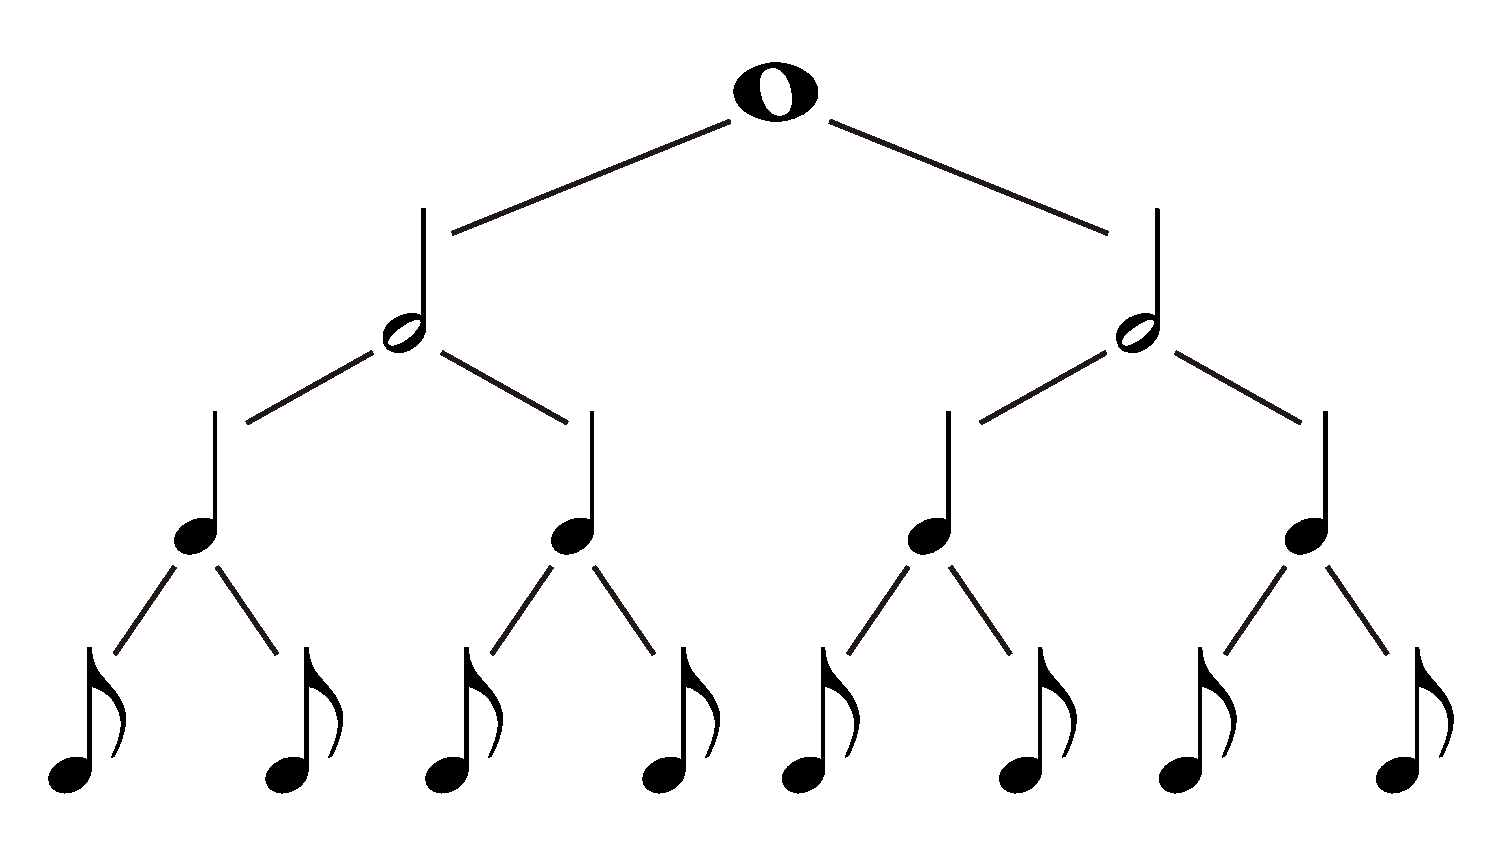
\includegraphics[width=0.8\linewidth]{imagenes/music_tree.pdf}
	\caption{Diagrama de subdivisión de figuras}
	\label{fig:subdivision-figuras}
\end{figure}

Dado que en inglés estas figuras se llaman mediante el nombre de la fracción de redonda que representan también pueden ser representadas mediante el número del denominador de dicha fracción. De este modo la redonda sería 1, la blanca 2, la negra 4, la corchea 8, la semicorchea 16, etc. A mayores existen modificadores de la duración de las figuras como el puntillo, un pequeño punto situado a la derecha de las figuras que alarga la duración de las mismas durante la mitad de la duración de la figura a la que acompaña.

El \textit{tempo}, anteriormente mencionado, es una relación que indica la cantidad aproximada de figuras de negra que suenan en un minuto, debido a eso la magnitud que representa el \textit{tempo} se denomina BPM o \textit{Blacks per Minute}.

\begin{figure}[hpt]
	\centering
	\begin{music}
		\largemusicsize
		\setlines1{1}
		\setclefsymbol1\empty
		\nobarnumbers
		\startextract                      % starting real score
		\Notes\wh i\hu i\qu i\cu i\en\bar
		\Notes\pause \hpause \qp \ds \en
		\setdoublebar\stoppiece
		\zendextract                       % terminate excerpt
	\end{music}
	\caption{Figuras con sus respectivos silencios, de izquierda a derecha: Redonda, blanca, negra, corchea}
	\label{fig:figuras}
\end{figure}

La partitura está dividida en compases, y al principio de la pieza se indica el tipo de compás de la misma. Se representa con dos números colocados en vertical que indican respectivamente la cantidad de figuras que caben en cada compás y el tipo de dicha figura, utilizando el sistema del numerador de la fracción de redonda detallado anteriormente. A modo de aclaración, el tipo de figura utilizado en el compás solamente indica la figura base del mismo, pero eso no impide que se utilicen fracciones o figuras de mayor longitud equivalentes siempre y cuando se respete que la suma de sus duración no supere la especificada en el tipo de compás. 

Según la cantidad de figuras que caben en cada compás, estos reciben diferentes nombres. En la música moderna lo más habitual es encontrar compases cuaternarios, aunque en algunas corrientes de la música clásica como el \textit{Waltz} predominan los ternarios. 

\begin{figure}[hpt]
	\centering
	\begin{music}
		\largemusicsize
		\setlines1{1}
		\setclefsymbol1\empty
		\generalmeter{\meterfrac{4}{4}}%
		\nobarnumbers
		\startextract                      % starting real score
		\Notes\cu i\hu i\qu i\cu i\en
		\generalmeter{\meterfrac{3}{4}}\changecontext
		\Notes\qu i\hu i\en
		\setdoublebar\stoppiece
		\zendextract                       % terminate excerpt
	\end{music}
	\caption{Ejemplos de tipos de compases: Cuaternario y Ternario}
	\label{fig:compas}
\end{figure}

El acento en la música es un mero hincapié interpretativo en los tiempos fuertes de la pieza. Aunque puede existir una acentuación arbitraria a lo largo de la partitura, los compases determinan además los tiempos fuertes y normalmente acentuados. Dependiendo del tipo de compás estos varían, aunque la primera figura de cada compás suele estar acentuada y ser considerada fuerte. No obstante, la diferenciación de tiempos débiles y fuertes es importante en la melodía y por tanto en la armonía, por ello se revisará este concepto en los puntos siguientes.


\subsection{Melodía y pentagrama}

La melodía de la pieza es la secuencia de notas que siguen las diferentes voces a lo largo de la partitura. Para ello se utilizan siete notas fundamentales diferentes: Do, Re, Mi, Fa, Sol, La y Si (C, D, E, F, G, A, B en la notación internacional). Entre cada uno de estas notas fundamentales se establece una distancia de un tono, excepto entre Si y Do; y entre Mi y Fa, entre las cuales sólo hay medio tono (también denominado semitono). Las fundamentales pueden ser alteradas mediante modificaciones conocidas como Sostenido y Bemol, que suben o bajan, respectivamente, un semitono a dichas notas, por eso podemos entender que contamos, en total, con 12 sonidos distintos.

Estas siete notas fundamentales (o doce sonidos), tienen asociadas a su vez una octava. Cada octava es un conjunto formado por esos mismos sonidos pero en un registro más agudo o más grave. Si bien esto produce un sonido diferente, el mismo sonido de diferentes octavas es, de mdo general, equivalente en términos de armonía.

La representación de estos sonidos se hace sobre un pentagrama, bandas formadas por cinco líneas con sus respectivos cuatro huecos donde pueden colocarse las notas de la partitura, representando cada línea y hueco consecutivos una nota fundamental diferente. Ya que esto solo permitiría representar nueve notas, se pueden utilizar líneas y huecos adicionales situados encima y debajo del pentagrama para indicar notas más graves o más agudas. En conjunción con las alteraciones ya mencionadas (Sostenido y Bemol) en un mismo pentagrama pueden representarse más de una veintena de sonidos diferentes. 

Para poder interpretar el sonido correspondiente a cada línea o hueco existe la clave. La clave es un símbolo situado al principio de cada pentagrama e indica la nota correspondiente a una de las cinco líneas. El resto se calculan subiendo o bajando huecos y renglones a partir de esa línea. 

\begin{figure}[h!]
	\centering
	\begin{music}
		\largemusicsize
		\generalmeter{\meterfrac{4}{4}}%
		\nobarnumbers
		\startextract                      % starting real score
		\Notes\qu {abcd}\en
		\setclef1\bass\changecontext
		\Notes\qu {abcd}\en
		\setdoublebar\stoppiece
		\zendextract                       % terminate excerpt
	\end{music}
	\caption{La misma secuencia de notas en clave de Sol y de Fa}
	\label{fig:claves}
\end{figure}

En la Figura \ref{fig:claves}, la clave de Sol indica que en la segunda línea, contando desde abajo, estaría ubicada la nota sol, mientras que la clave de Fa indica que en la cuarta línea, contando también desde abajo, se ubicaría el sonido Fa. La finalidad de las diferentes claves es ofrecer diferentes puntos de referencia, ya que no solo indican nota sino también octava, evitando así sobrecargar la partitura con notas fuera de las cinco líneas principales. La clave de Sol utiliza sonidos más agudos, mientras que la de Fa utiliza sonidos más graves. Es habitual encontrar, por ejemplo, partituras para piano donde la mano izquierda estará escrita en clave de Fa al ser notas más graves y en clave de Sol la de la mano derecha, al ser notas más agudas. 

La transposición es un proceso mediante el cual una nota es desplazada una cantidad de semitonos hacia arriba o hacia abajo. Aplicado a una sección de una pieza musical, todas las notas de dicha sección subirían o bajarían la misma cantidad de semitonos especificada.

Un salto melódico es la diferencia de frecuencia entre dos sonidos consecutivos de una misma melodía. De este modo, si el siguiente sonido es más agudo se producirá un salto ascendente, y si es más grave, descendente. Las secuencias ascendentes y descendentes se combinan con el ritmo de la canción para crear tramos de tensión melódica, de resolución, de reposo... Para entender estos conceptos es necesario introducir el concepto de escala. 

\begin{figure}[h!]
	\centering
	\begin{music}
		\largemusicsize
		\nobarnumbers
		\startextract                      % starting real score
		\Notes\cu {cdefghij}\en
		\setdoublebar\stoppiece
		\zendextract                       % terminate excerpt
	\end{music}
	\begin{music}
		\largemusicsize
		\nobarnumbers
		\startextract                      % starting real score
		\Notes\cu {cd_efg_h_ij}\en
		\setdoublebar\stoppiece
		\zendextract                       % terminate excerpt
	\end{music}
	\label{fig:escalas}
	\caption{Escalas de Do Mayor y Do Menor}
\end{figure}

Una escala es un subconjunto de los doce sonidos disponibles donde sus miembros cumplen una distribución concreta de separaciones tonales. La escala más conocida es la de Do Mayor, ya que empezando desde Do, pasa por las siete notas fundamentales, pero si se mira de desde la distribución de tonos y semitonos entre sus notas (Tono, Tono, Semitono, Tono, Tono, Tono, Semitono) se puede construir cualquier otra escala mayor dada una nota arbitraria de partida. Las escalas pueden ser, según su distribución tonal Mayores o Menores, así como recibir diferentes nombres según la cantidad de sonidos que incluyan. La escala de Do Mayor es en realidad la escala Heptatónica de Do Mayor ya que incluye siete sonidos, pero otras escalas como las Pentatónicas también son frecuentemente utilizadas en la música moderna. La escala sobre la que se construye una pieza puede ser denominada tonalidad y recibe el nombre de la nota raíz junto con su modo, así una pieza construida con la escala de Do Mayor puede decirse que está en tonalidad de Do Mayor.

En aquellas piezas en las que se trabaja con una determinada tonalidad, resulta cómodo especificar una armadura. La armadura es un conjunto de alteraciones al principio del pentagrama, justo a la derecha de la clave, que indica qué alteraciones tendrán las notas de ese pentagrama a lo largo de toda la canción o hasta que se especifique lo contrario. De este modo, para la escala de Do Menor de la Figura \ref{fig:escalas} podría especificarse una armadura que indicase tres bemoles en las líneas de mi, la y si. Si quisiéramos escribir esas notas sin la alteración, para contrarrestar la armadura, habría que usar otra alteración denominada becuadro. El becuadro, también conocido como natural, elimina las alteraciones establecidas por la armadura del pentagrama. Esta armadura no solo resulta conveniente para el compositor, al tener que escribir las alteraciones de la snotas una única vez al comienzo, sino que también es muy útil a la hora de identificar la tonalidad de la pieza, ya que suele ser un indicativo fiable de la misma.

\begin{figure}[h]
	\centering
	\begin{music}
		\largemusicsize
		\nobarnumbers
		\startextract                      % starting real score
		\Notes\cu {cd_efg_h_ij}\en
		\setdoublebar\stoppiece
		\zendextract                       % terminate excerpt
	\end{music}
	\begin{music}
		\largemusicsize
		\nobarnumbers
		\setsign1{-3}
		\startextract                      % starting real score
		\Notes\cu {cdefghij}\en
		\setdoublebar\stoppiece
		\zendextract                       % terminate excerpt
	\end{music}
	\caption{Escala de Do Menor sin armadura y con armadura}
	\label{fig:armadura}
\end{figure}

\subsection{Armonía}

Si la melodía es la sucesión de notas en el tiempo, se puede entender la armonía como los conjuntos de notas que suenan a la vez a lo largo de un intervalo de tiempo. Por eso se habla de que el análisis melódico es horizontal y el armónico vertical, aunque esto no es del todo cierto, pues al fin y al cabo la armonía analiza también intervalos horizontales de tiempo (normalmente acotados en compases) y la estructura general de la pieza. Para poder estudiar o crear armonía se debe contar siempre o bien con varias voces o bien con instrumentos polifónicos capaces de producir sonidos simultáneos (Como el Piano o la Guitarra)

Uno de los conceptos más importantes dentro de la armonía es la tonalidad. La armonía define siete grados para una tonalidad, y están relacionados con la escala de dicha tonalidad. Cada grado está referido a cada una de las notas de las calas y se representa mediante un número romano de forma consecutiva, además de un nombre. Los grados más relevantes son el I, IV y V, mientras que los menos importantes o débiles son el II y el VI. A mayores, los grados muy débiles son el III y el VII.

\begin{itemize} 
	\item I (Tónica)
	\item II (Supertónica)
	\item III (Mediante)
	\item IV (Subdominante)
	\item V (Dominante)
	\item VI (Superdominante/Submediante)
	\item VII (Sensible)
\end{itemize}

Según la teoría, un acorde son tres o más sonidos simultáneos a una distancia de tercera entre sí de forma ascendente. Analizando el tercer grado de la escala de las notas del acorde, podemos determinar si este es mayor o menor. La nota generadora del acorde suele ser la tónica y además la más grave del mismo, si no es así se dice que el acorde está invertido.

\begin{figure}[h!]
	\centering
	\begin{music}
		\largemusicsize
		\nobarnumbers
		\startextract                      % starting real score
		\Notes\zq{ce}\qu g\en
		\Notes\zq{df}\qu h\en
		\Notes\zq{eg}\qu i\en
		\Notes\zq{fh}\qu j\en
		\Notes\zq{gi}\qu k\en
		\Notes\zq{hj}\qu l\en
		\Notes\zq{ik}\qu m\en
		\setdoublebar\stoppiece
		\zendextract                       % terminate excerpt
	\end{music}
	\caption{Acordes de la tonalidad de Do Mayor}
	\label{fig:acordes}
\end{figure}

En una escala de modo mayor, el I, IV y V grado son acordes perfectos mayores, el II, III y VI acordes perfectos menores, y el VII un acorde disminuido. En una escala de modo menor, el I y IV grado son acordes perfectos menores, el II y VII son acordes disminuidos, el III es aumentado.

Ciertas combinaciones de acordes producen sensación de tensión, mientras que otras producen sensación de reposo. Algunos acordes, según el contexto, tienen un sentido conclusivo y otros, un sentido transitorio. Estos conceptos son muy importantes en composición, así como en armonización.

La armonización es el proceso de construir una armonía mediante varias voces que, sin modificar la melodía de la pieza, enriquezca la misma reforzando la tonalidad en cada instante. Esto se consigue identificando la tonalidad de la pieza en cada tramo, tomando las notas del mismo y averiguando la escala sobre la que se ha construido la melodía. Dada la escala podemos identificar la tonalidad, y con la tonalidad construir por fin los acordes. 

\begin{figure}[h]
	\centering
	\begin{music}\nostartrule
		\parindent10mm
		\nobarnumbers
		\instrumentnumber{1}       % a single instrument
		\setname1{Piano}           % whose name is Piano
		\setstaffs1{2}             % with two staffs
		\generalmeter{\meterfrac44}% 4/4 meter chosen
		\startextract              % starting real score
		\Notes\ibu0f0\qb0{cge}\tbu0\qb0g|\hl j\en
		\Notes\ibu0f0\qb0{cge}\tbu0\qb0g|\ql l\sk\ql n\en
		\bar
		\Notes\ibu0f0\qb0{dgf}|\qlp i\en
		\notes\tbu0\qb0g|\ibbl1j3\qb1j\tbl1\qb1k\en
		\Notes\ibu0f0\qb0{cge}\tbu0\qb0g|\hl j\en
		\setdoublebar\stoppiece
		\zendextract                 % terminate excerpt
	\end{music}
	\caption{Ejemplo de polifonía para Piano (Sonata en Do Mayor, Mozart)}
	\label{fig:polifonia}
\end{figure}

No obstante, existen reglas a respetar, ya que no es tan sencillo como tomar cada nota de la melodía como nota generadora de un acorde y construir el acorde mayor o menor correspondiente a la misma. Por otra parte no basta con tocar el acorde principal de la tonalidad a lo largo de toda la pieza, ya que si bien esto no sería erróneo, podría producir problemas con las fluctuaciones de la melodía, y no cumpliría, en último extremo, la finalidad de enriquecer la melodía.

Los acordes no solo deben respetar la melodía, sino que además deben ser escogidos de tal forma que se enlacen correctamente, normalmente debido a las notas compartidas entre dos acordes consecutivos. Las notas distintas al enlazar dos acordes pueden producir sonidos indeseados con respecto a la melodía o causar saltos melódicos no agradables al oído. Para evitar estos problemas se estudia a su vez, horizontalmente, las nuevas líneas melódicas formadas por las diferentes voces de los acordes. Los diferentes movimientos de estas voces podrían ser, entre otros:

\begin{itemize} 
	\item Paralelo: Dos voces de varios acordes siguiendo una distancia, realizando los mismos saltos melódicos.
	\item Oblicuo: Una voz representada con una nota de larga duración y otra voz moviéndose libremente.
	\item Directo: Dos voces moviéndose a la vez de forma ascendente o descendente, pero no en paralelo.
	\item Contrario: Dos voces moviéndose en sentidos distintos.
\end{itemize}

En movimientos como el paralelo o el contrario pueden surgir problemas armónicos, como formar un intervalo de octava o quinta justa sobre las mismas voces. El movimiento directo también presenta problemas armónicos, en voces extremas (Bajo y Soprano), si la voz de la Soprano (más aguda) no se mueve por grados conjuntos, se presenta ese problema. En partes intermedias (voces centrales o una voz central y otra extrema), si una de esas dos voces no se mueve por grados conjuntos, ese enlace sería incorrecto. En voces seguidas, se busca evitar los saltos de octava



